% !TEX encoding = UTF-8 Unicode
%%%%%%%%%%%%%%%%%%%%%%%%%%%%%%%%%%%%%%%%%%%%%%%%%%%%%%%%%%%%%%%%%%%%%%%%%%%%%%%%%%%%%%%%%%%%%%%%%%%%%%% 
%%
%%  This file is asmeconf-template.tex, a LaTeX template to format ASME Conference papers according to
%%  the requirements on ASME's conference web pages, and including hypertext support for the pdf.
%%
%%  This file is version 1.30 dated 2022/03/14
%%  
%%  As of version 1.11, this template defaults to ASME's newer conference guidelines first posted July 2019.
%% 			Those guidelines changed the requested author block formatting to be inline. 
%%			This LaTeX template continues to support the traditional grid format as a package option, [grid].
%%			Nomenclature now follows the abstract. Abstract text is set in italics.
%%
%%  Author: John H. Lienhard V
%%          Department of Mechanical Engineering
%%          Massachusetts Institute of Technology
%%          Cambridge, MA 02139-4307 USA
%%
%%  Class options include:
%%
%%          * Math options from M. Sharpe's newtxmath package: upright integrals [upint]; 
%%          *    [varvw] for a v and w that are better distinguished from Greek nu; and also 
%%          *    [subscriptcorrection, smallerops, varg, frenchmath, varbb, cmbraces, slantedGreek,...] 
%%			* 	 See newtx documentation for descriptions (at CTAN: http://ctan.org, v1.6 or higher is best).
%%
%%          * Options to: 	omit the ASME copyright footer [nofoot]; 
%%			*				use government employee copyright notice [govt];
%%			*				use government contractor copyright notice [contractor]
%%
%%          * An option to use the traditional grid arrangement of author names [grid].  
%%			*	 With this option, line breaks (\\) may be inserted into the address as needed. 
%%			*	 Author names that include commas should be enclosed in braces, e.g., {Joseph L. Smith, Jr.}.  
%%			*	 Authors may be grouped above a single affiliation using braces, e.g., {Henry Tudor, Catherine Parr}.
%%
%%          * An option to balance the heights of columns on the last page [balance]. 
%%          *    This option is NOT compatible with the [lineno] option.
%%
%%          * An option to include line numbers [lineno]. You must *run twice* for proper placement of the line numbers. 
%%			*	 The lineno package does not number titles, footnotes, captions, or tables.
%%          *    This option will disable balancing column height on final page if that option has been invoked.
%%          *    The lineno package won't always number the lines preceding displayed math in a paragraph because
%%          *    paragraph has not ended.  See that package's documentation for macros to address this problem, or
%%          *    just leave a blank line above the displayed equation while you are editing and then remove the 
%%          *    blank line and [lineno] option when you move to your final version.
%%
%%			* Options for PDF/A compliance. [pdf-a] will produce PDF/A-3u compliance with sRGB OutputIntent.
%%			*	 [pdfapart= 1 or 2 or 3] and [pdfaconformance= b or u] can enable levels 1b, 2b, 2u, and 3b.
%%			*    The most recent versions of LaTeX (2021 and later) are moving toward integrated support for pdf-a, 
%%			*    through \DeclareDocumentMetadata{..}. The asmeconf class supports these new features, which can 
%%			*	 replace the aforementioned class options. (An up-to-date LaTeX installation is required to use this.)
%%
%%          * Many options for calligraphic, script, and fraktur fonts from the mathalfa package; the
%%          *    example shown here is: [mathalfa=cal=boondoxo] to use a Boondox font for \mathcal.
%%          *    Some other options for cal are: dutchcal, zapfc, cm (default), euler,...
%%          *    frak (fraktur), bb (blackboard bold), scr (script) may also be chosen this way.
%%			*	 For details, refer to mathalfa documentation (at CTAN: http://ctan.org).
%%
%%          * Option to use superiors font from newtxtext for footnotes [nodefaultsups] and
%%          *    for slightly larger small capitals, [largesc], also from newtxtext.
%%
%%          * An option to allow hyphenation of the typewriter font [hyphenate], from inconsolata package.
%%          *    Hyphenation is normally suppressed for typewriter mode because it is often used for code.
%%			*	 To replace the default variable word spacing by monospacing, use the option [mono].
%%			*	 To get a zero without a slash, use [var0]
%%
%%          * Options (used by the babel package) to include passages in languages other than English (e.g., a translation 
%%			*    of the abstract). Languages are called as options, e.g. [french], [spanish], [greek], [russian], etc. 
%%			*    Language support is greatest when running LuaLaTeX with the [fontspec] option.
%%			*    See Appendix B for details.
%%
%%  The use of commands defined or modified by the asmeconf class is illustrated throughout this file. In particular, 
%%  ASME requires capitalized, sans-serif section headings, and as a result some care is needed when using macros 
%%  in section headings, as also illustrated below.
%%
%%  Use an up-to-date and complete installation of LaTeX, such as TeX Live 2020 or later. Errors may occur with old set-ups.
%%
 %=========================================================
%% 
%% LICENSE: 
%%
%% Copyright (c) 2022 John H. Lienhard
%%
%% Offered under the MIT license: https://ctan.org/license/mit 
%%
%%%%%%%%%%%%%%%%%%%%%%%%%%%%%%%%%%%%%%%%%%%%%%%%%%%%%%%%%%%%%%%%%%%%%%%%%%%%%%%%%%%%%%%%%%%%%%%%%%%%%%% 

%% New pdf management code (June 2021); with this, the class option [pdf-a] can be omitted.
%% This change to the LaTeX kernel is being phased-in by the LaTeX3 team. Can delete if it gives you trouble.
%% Under LuaLaTeX, choose pdfstandard=A-3b (and be cautious when loading extra fonts)

%\RequirePackage{pdfmanagement-testphase}%
%   \DocumentMetadata{%
%		pdfstandard=A-3b,% A-2b, A-2u, A-3b, or A-3u
%		pdfversion=1.7,
%		lang=en-US,
%	}%

%%%%%%%%%%%%%%%%%%%%%%%%%%%%%%%%%%%%%%%%%%%%%%%%%%%%%%%%%%%%%%%%%%%%%%%%%%%%%%%%%%%%%%%%%%%%%%%%%%%%%%%

%% Class options are described above. Change these options as desired. 
%%		If you are not using the language options, remove them (together with Appendices B and C)
%%	 	Remove the [colorlinks] option before *final* submission to ASME, to get black text for printing,
%%		but keep that option for other uses.
 
\documentclass[balance,upint,subscriptcorrection,varvw,nofoot, mathalfa=cal=boondoxo,spanish,french,vietnamese,russian,greek,pdf-a,fontspec,colorlinks]{asmeconf}
%%%%%  pdf metadata  %%%%%%%%%%%%%%%%%%%%%%%%%%%%%%%%%%%%%%%%%%%%%%%%%%%%%%%%%%%%%%%%%%%%%%%%%%%%%%%%%%
\hypersetup{%
	pdfauthor={John H. Lienhard},                       		      % <=== change to YOUR name[s]!
	pdftitle={ASME Conference Paper LaTeX Template},                  % <=== change to YOUR pdf file title
	pdfkeywords={ASME conference paper, LaTeX template, BibTeX style},% <=== change to YOUR pdf keywords
	pdfsubject = {Describes the asmeconf LaTeX template},			  % <=== change to YOUR subject
%	pdfurl={https://ctan.org/pkg/asmeconf},% may delete
	pdflicenseurl={https://ctan.org/pkg/asmeconf},% may delete
}

%%%%%%%%%%%%%%%%%%%%%%%%%%%%%%%%%%%%%%%%%%%%%%%%%%%%%%%%%%%%%%%%%%%%%%%%%%%%%%%%%%%%%%%%%%%%%%%%%%%%%%%
\usepackage{minted}
\makeatletter
\@namedef{T1/zi4/m/it}{<->ssub*zi4/m/n}
\begin{document}

% Change these fields to the right content for your conference.
% You can comment these out if for some reason you don't want a header.
% Use title case (first letters capitalized), not all capitals

% \ConfName{Proceedings of the ASME 2022\linebreak International Mechanical Engineering Congress and Exposition}
% \ConfAcronym{IMECE2022}
% \ConfDate{October 30--November 3, 2022} % update 
% \ConfCity{Columbus, OH} % update 
% \PaperNo{IMECE2022-XXXX}

% Units of measure (e.g., cm) and other specialty lowercase terms in the title should be 
%   enclosed in \NoCaseChange{...} to maintain lower case type
%   LaTeX will automatically set the rest of the title in all capital letters.

\title{Stereo Camera and Solid State Lidar Object Detection on Small Delivery Robot} % <=== replace with YOUR title
%\title{Place Title Here: Place Subtitle After Colon} 
 
%   Put author names into the order you want. Use the same order for affiliations.
%   \affil{#} tags the author's affiliation to the address in \SetAffiliation{#}.
%   No space between last name and \affil{#}, separate names with commas.
%
%	For a sole author or a single affiliation for all authors, {#} may be left empty, as \affil{} and \SetAffiliation{} (but not with [grid] option!)
%
%   \CorrespondingAuthor{email} follows that author's affiliation, no spaces.  
%   If multiple corresponding authors, put both email addresses in the same command and place after both authors.
%
%   \JointFirstAuthor, if applicable, follows the affiliation of the relevant authors, no spaces.

\SetAuthors{%
	Jiarun Wei\affil{1}\JointFirstAuthor, 
	Ding Zhao\affil{2}\JointFirstAuthor
	}

\SetAffiliation{1}{Carnegie Mellon University, Pittsburgh, PA}
\SetAffiliation{2}{Carnegie Mellon University, Pittsburgh, PA}

%	Note: Luis and Maria are not real people.  Henry and Catherine have been dead for >450 years.

%	To switch from inline author names to gridded names, use the [grid] option.

\maketitle

%%% Use this footnote for tracking various versions of your draft. Change text to suit your own needs. 
%%% \date{..} calls the same command. 
% \versionfootnote{Documentation for \texttt{asmeconf.cls}: Version~\versionno, \today.}% <=== Delete before final submission.


%%% Change these to your keywords.  Keywords are automatically printed at the end of the abstract.
%%% This command MUST COME BEFORE the end of the abstract.
%%% If you don't want keywords, leave the argument of \keywords{} empty (or use the abstract* environment)

\keywords{Object detection, Computer Vision, Solid-state Lidar, Autonomous Delivery}

%%%%%  End of fields to be completed. Now write your paper. %%%%%%%%%%%%%%%%%%%%%%%%%%%%%%%%%%%%%%%%%%%


%%%%%  ABSTRACT  %%%%%%%%%%%%%%%%%%%%%%%%%%%%%%%%%%%%%%%%%%%%%%%%%%%
%%
%% Abstract should be 200 words or less
\begin{abstract}

Stereo camera is popular in object detection due to its dense data. It works by matching
the key points of the left and right images, using the geometric constraints to calculate
the depth map, and then feed these into a neural network. Due to the geometric
constraints, it only works for a certain range of objects and is unstable for some objects.
Here we present a demo to stabilize the detection using solid state lidars, which is a very
cost efficient solution especially for small and slow robots.
\end{abstract}

%%%%%%%%%  NOMENCLATURE (OPTIONAL) %%%%%%%%%%%%%%%%%%%%%%%%%%%%%%%%%
%%
%% To change space between the symbols and  definitions, use \begin{nomenclature}[Xcm] where X is a number 
%% The unit cm can be replaced by any LaTeX unit of dimension: pt, in, ex, em, pc, etc.
%% Default is 2em.
%% \EntryHeading{..} produces an italicized subheading in the nomenclature list, e.g., \EntryHeading{Greek letters}




%%%%%%%%%  BODY OF PAPER %%%%%%%%%%%%%%%%%%%%%%%%%%%%%%%%%

\section{Introduction}
The main goal of this work is to stabilize the detection of objects using a stereo camera and lidar. 
The 
% \cite{DBLP:journals/corr/abs-1902-09738}

\section{Methods}

The stereo camera object detection can be decomposed into several parts: feature extraction, reigion proposal, reigion of intersection alignment, keypoint prediction and finally 3D bounding box estimation, which involves deep neural networks such as ResNet and binocular geometric constraints. In the following experiment, the lidar point clouds are used to verify the detection.
\paragraph{Feature extraction} The ResNet is one of the most commonly used feature extraction methods. Its architecture is shown in figure \ref{res}.
\begin{equation}
    \begin{aligned}
&v_{t}=\left(y-\frac{h}{2}\right) /\left(z-\frac{w}{2} \sin \theta-\frac{l}{2} \cos \theta\right) \\
&u_{l}=\left(x-\frac{w}{2} \cos \theta-\frac{l}{2} \sin \theta\right) /\left(z+\frac{w}{2} \sin \theta-\frac{l}{2} \cos \theta\right) \\
&u_{p}=\left(x+\frac{w}{2} \cos \theta-\frac{l}{2} \sin \theta\right) /\left(z-\frac{w}{2} \sin \theta-\frac{l}{2} \cos \theta\right) \\
&\quad \cdots \\
&u_{r}^{\prime}=\left(x-b+\frac{w}{2} \cos \theta+\frac{l}{2} \sin \theta\right) /\left(z-\frac{w}{2} \sin \theta+\frac{l}{2} \cos \theta\right)
\end{aligned}
\end{equation}

\paragraph{Reigion proposal}

\begin{figure}
\centering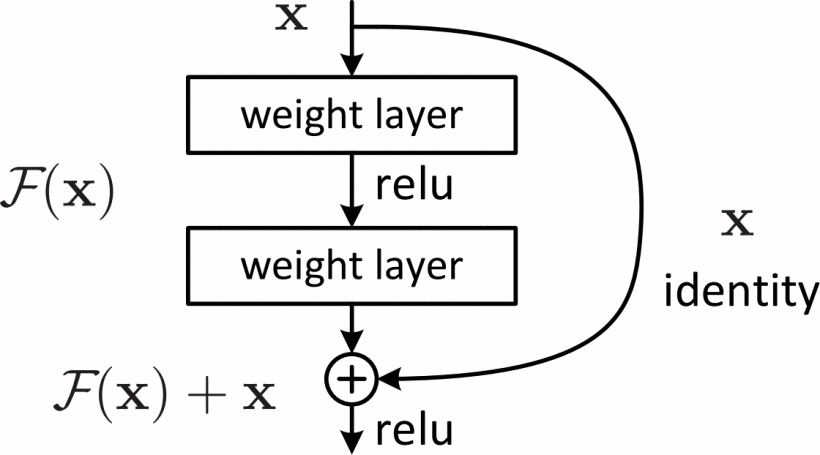
\includegraphics[width=0.7\linewidth]{resnet.png}
\caption{ResNet block}\label{res}
\end{figure}

%%%%%%%%%%%%%%%%%%%%%%%%%%%%%%%%%%%%%%%%%%%%%%%%%%%%%%%%%%%
\section{System Design}
As is shown in figure \ref{sys}, the delivery robot can be divided into 6 parts: stereo camera, router, battery, solid-state lidar and the processor. 
\paragraph{Stereo camera} The stereo camera is used for the detection of dynamic obstacles such as human and vehicles. Though the depth obtained by the stereo camera is not as accurate as the lidar, its object detection ability is a lot more better due to the RGB triple input channels.
\paragraph{Solid-state lidar} The lidar is used in multiple tasks: mapping, localization and object detection. 
\section{Experiment}

Figure 1 and 2 shows 2 views of the stereo camera object detection result of a person. The results are shown in blue bounding box with green vertices. The strips in the figures are the lidar point cloud. It is shown that the person in the bounding box is closely surrounded by the strips, which shows that the lidar point cloud overlaps with the camera object detection. Figure 3 shows the path planning result of the vehicle. The green line is the global planning path, the red line is the local planning path and the blue line is the localization.

%%%%%%%%%%%%% begin figure %%%%%%%%%%%%%%%%%

%% captions go below figures

\begin{figure}
\centering
\includegraphics[width=0.7\linewidth]{system.png}
\caption{System design}\label{sys}
\end{figure}

\begin{figure}
\centering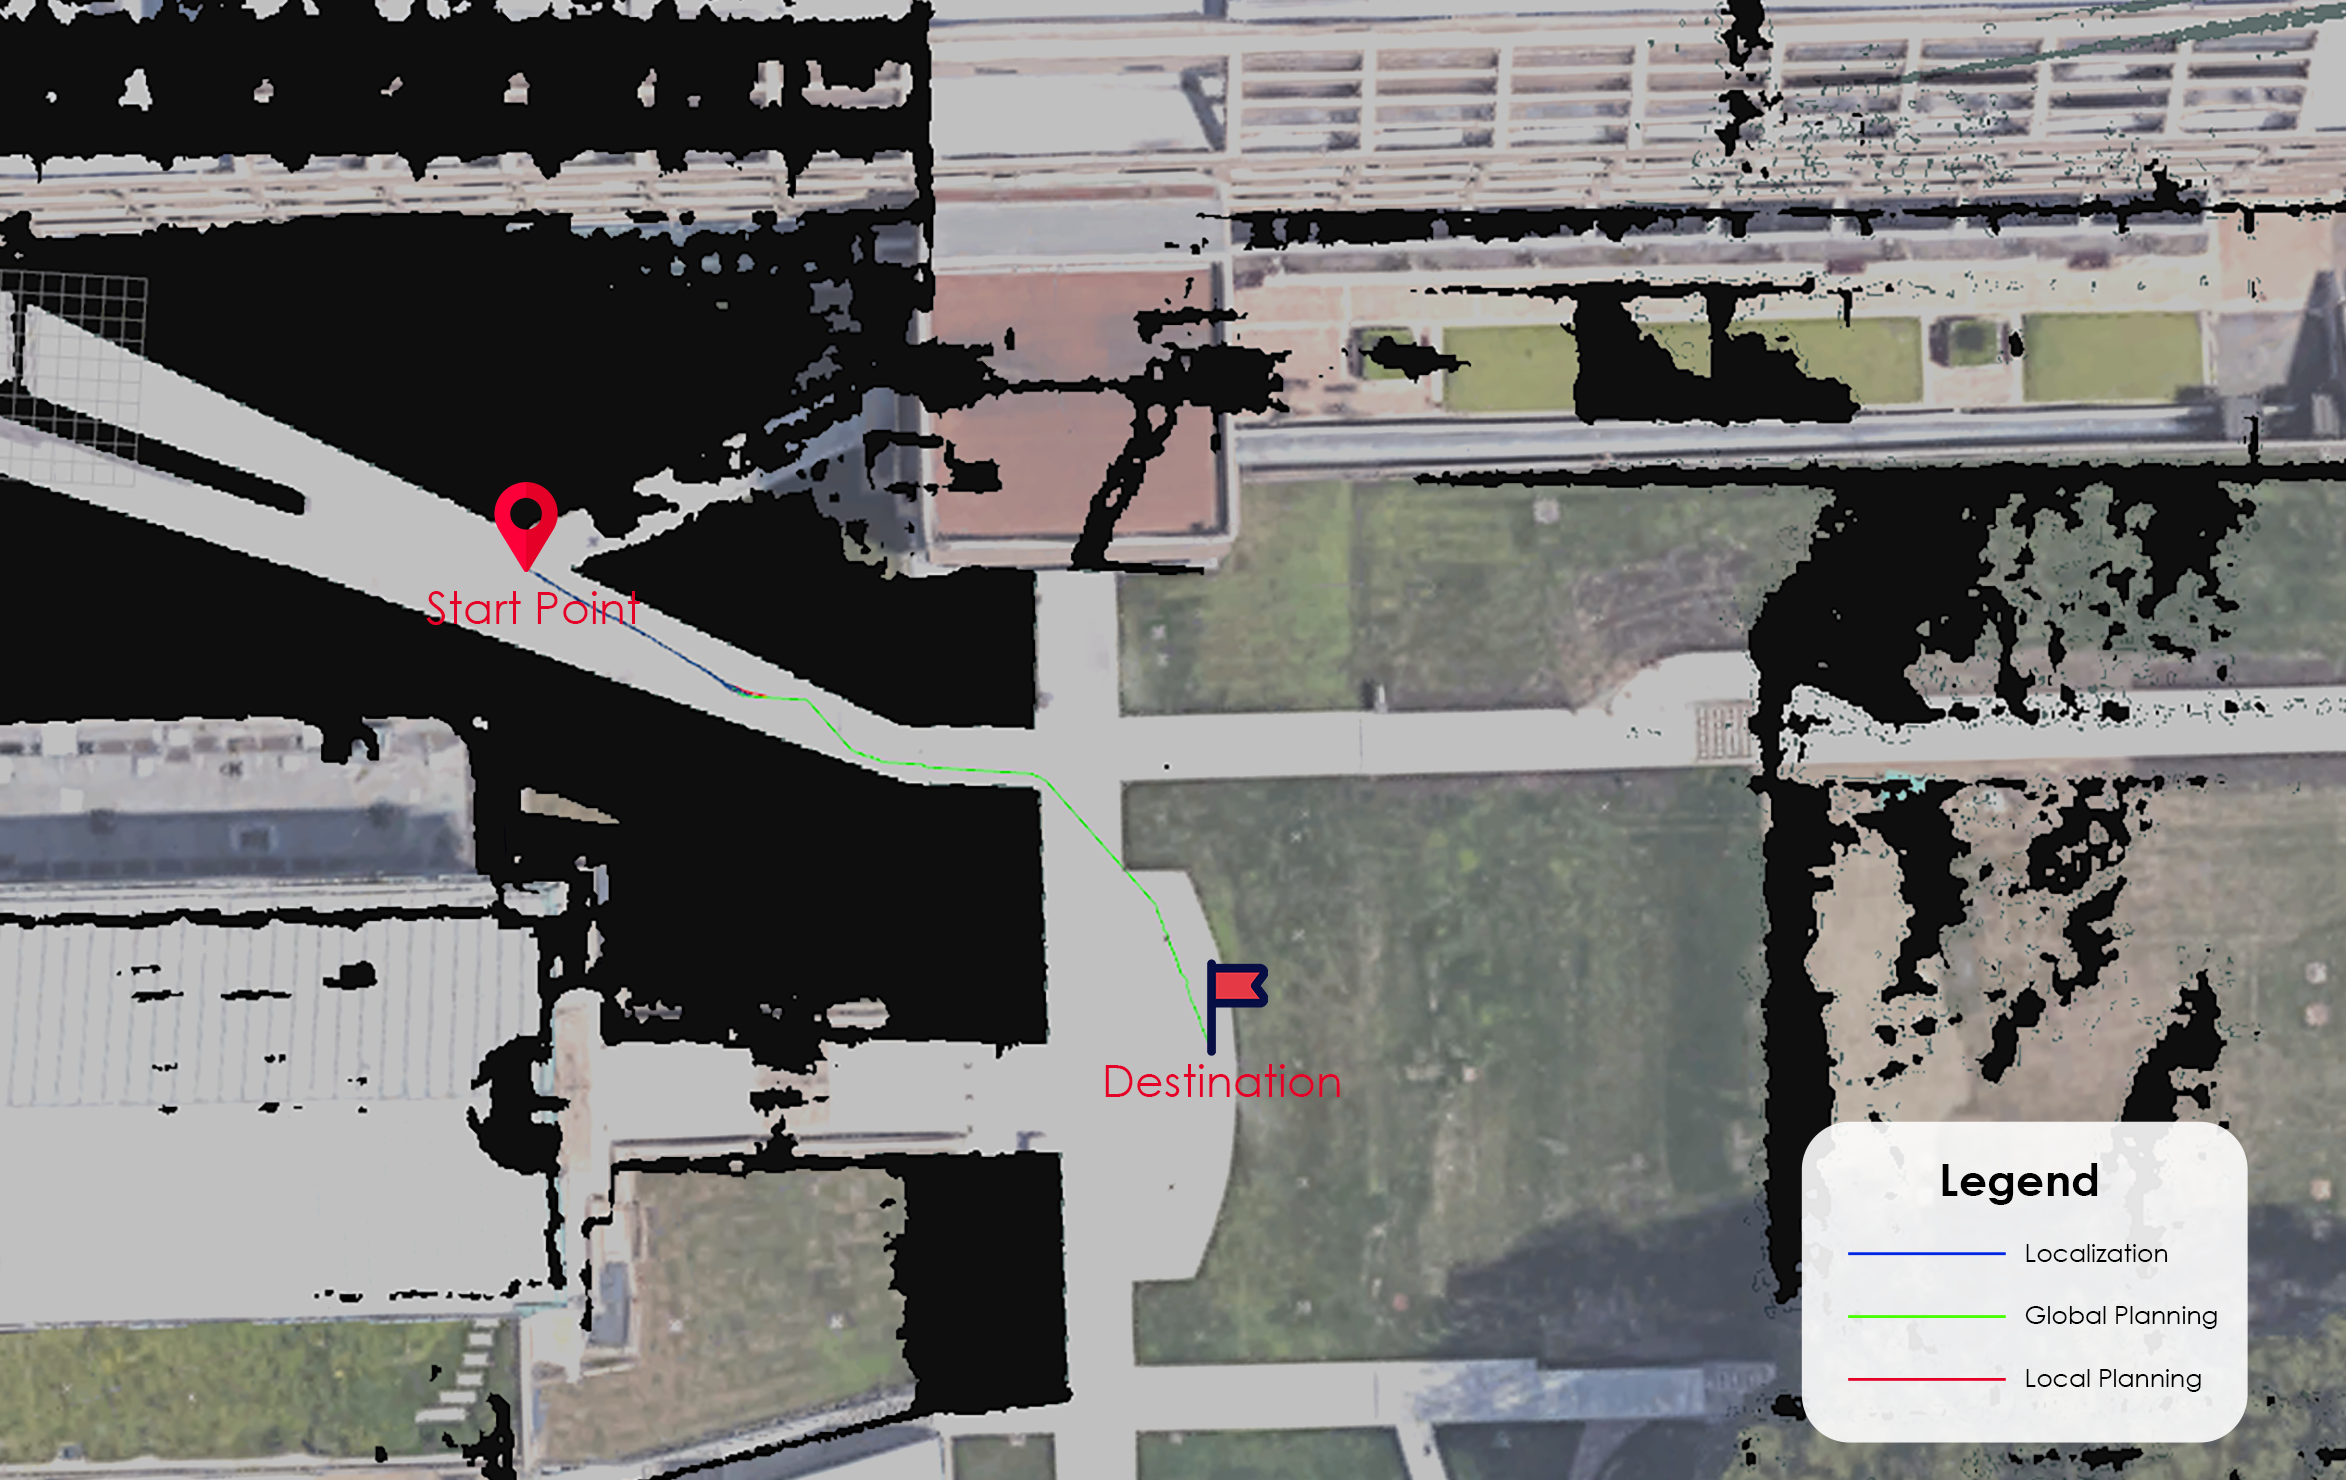
\includegraphics[width=0.7\linewidth]{Planning_psed.png}
\caption{Cost map}
\end{figure}
 
\begin{figure}
\centering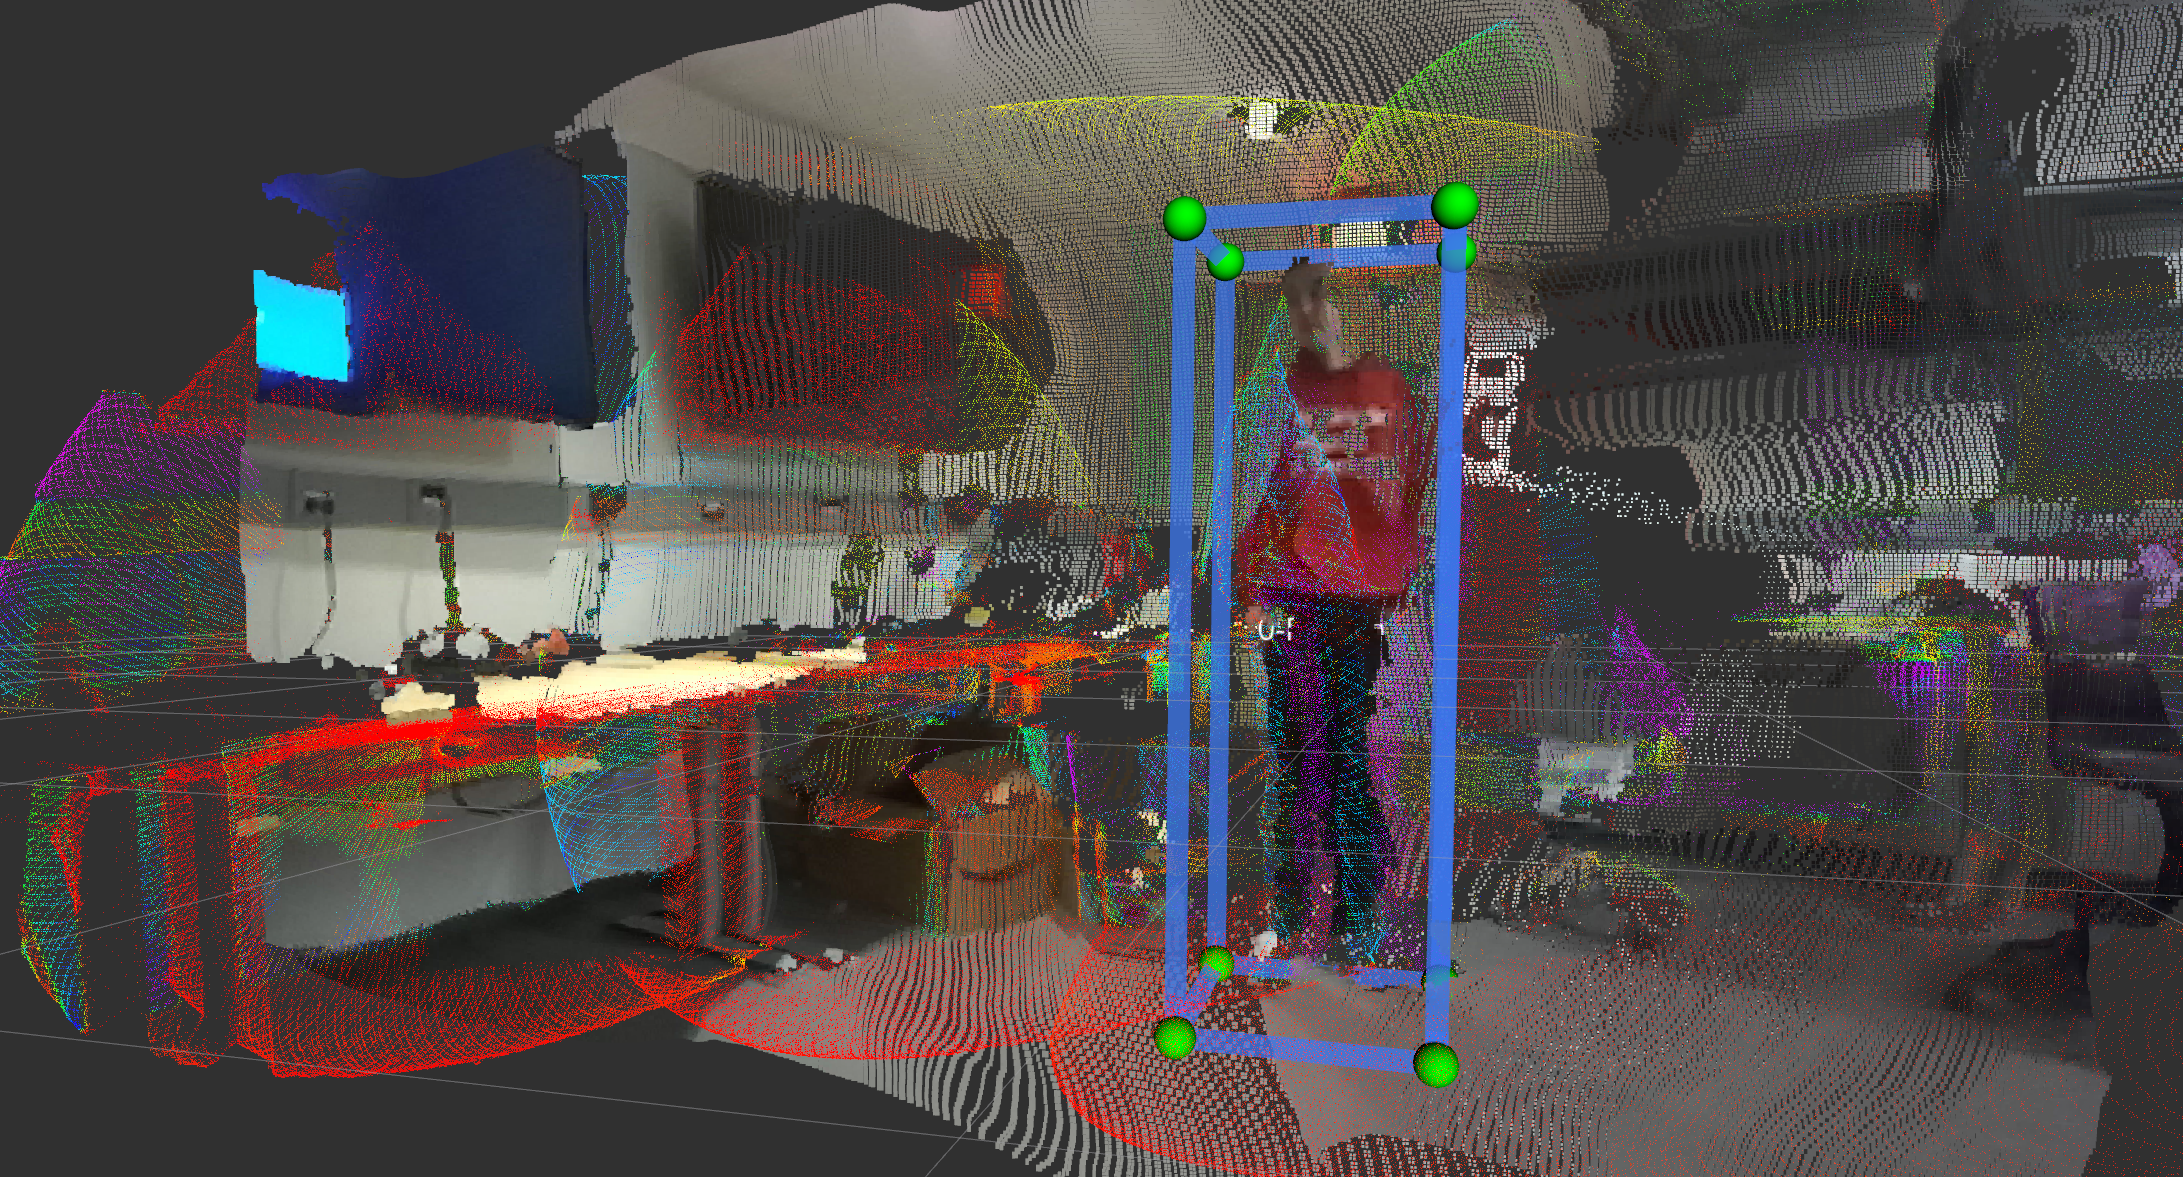
\includegraphics[width=0.7\linewidth]{obj_det.png}
\caption{Object detection verified by lidar}
\end{figure}

% \begin{multicols}{2}

\begin{figure*}[h]
\center
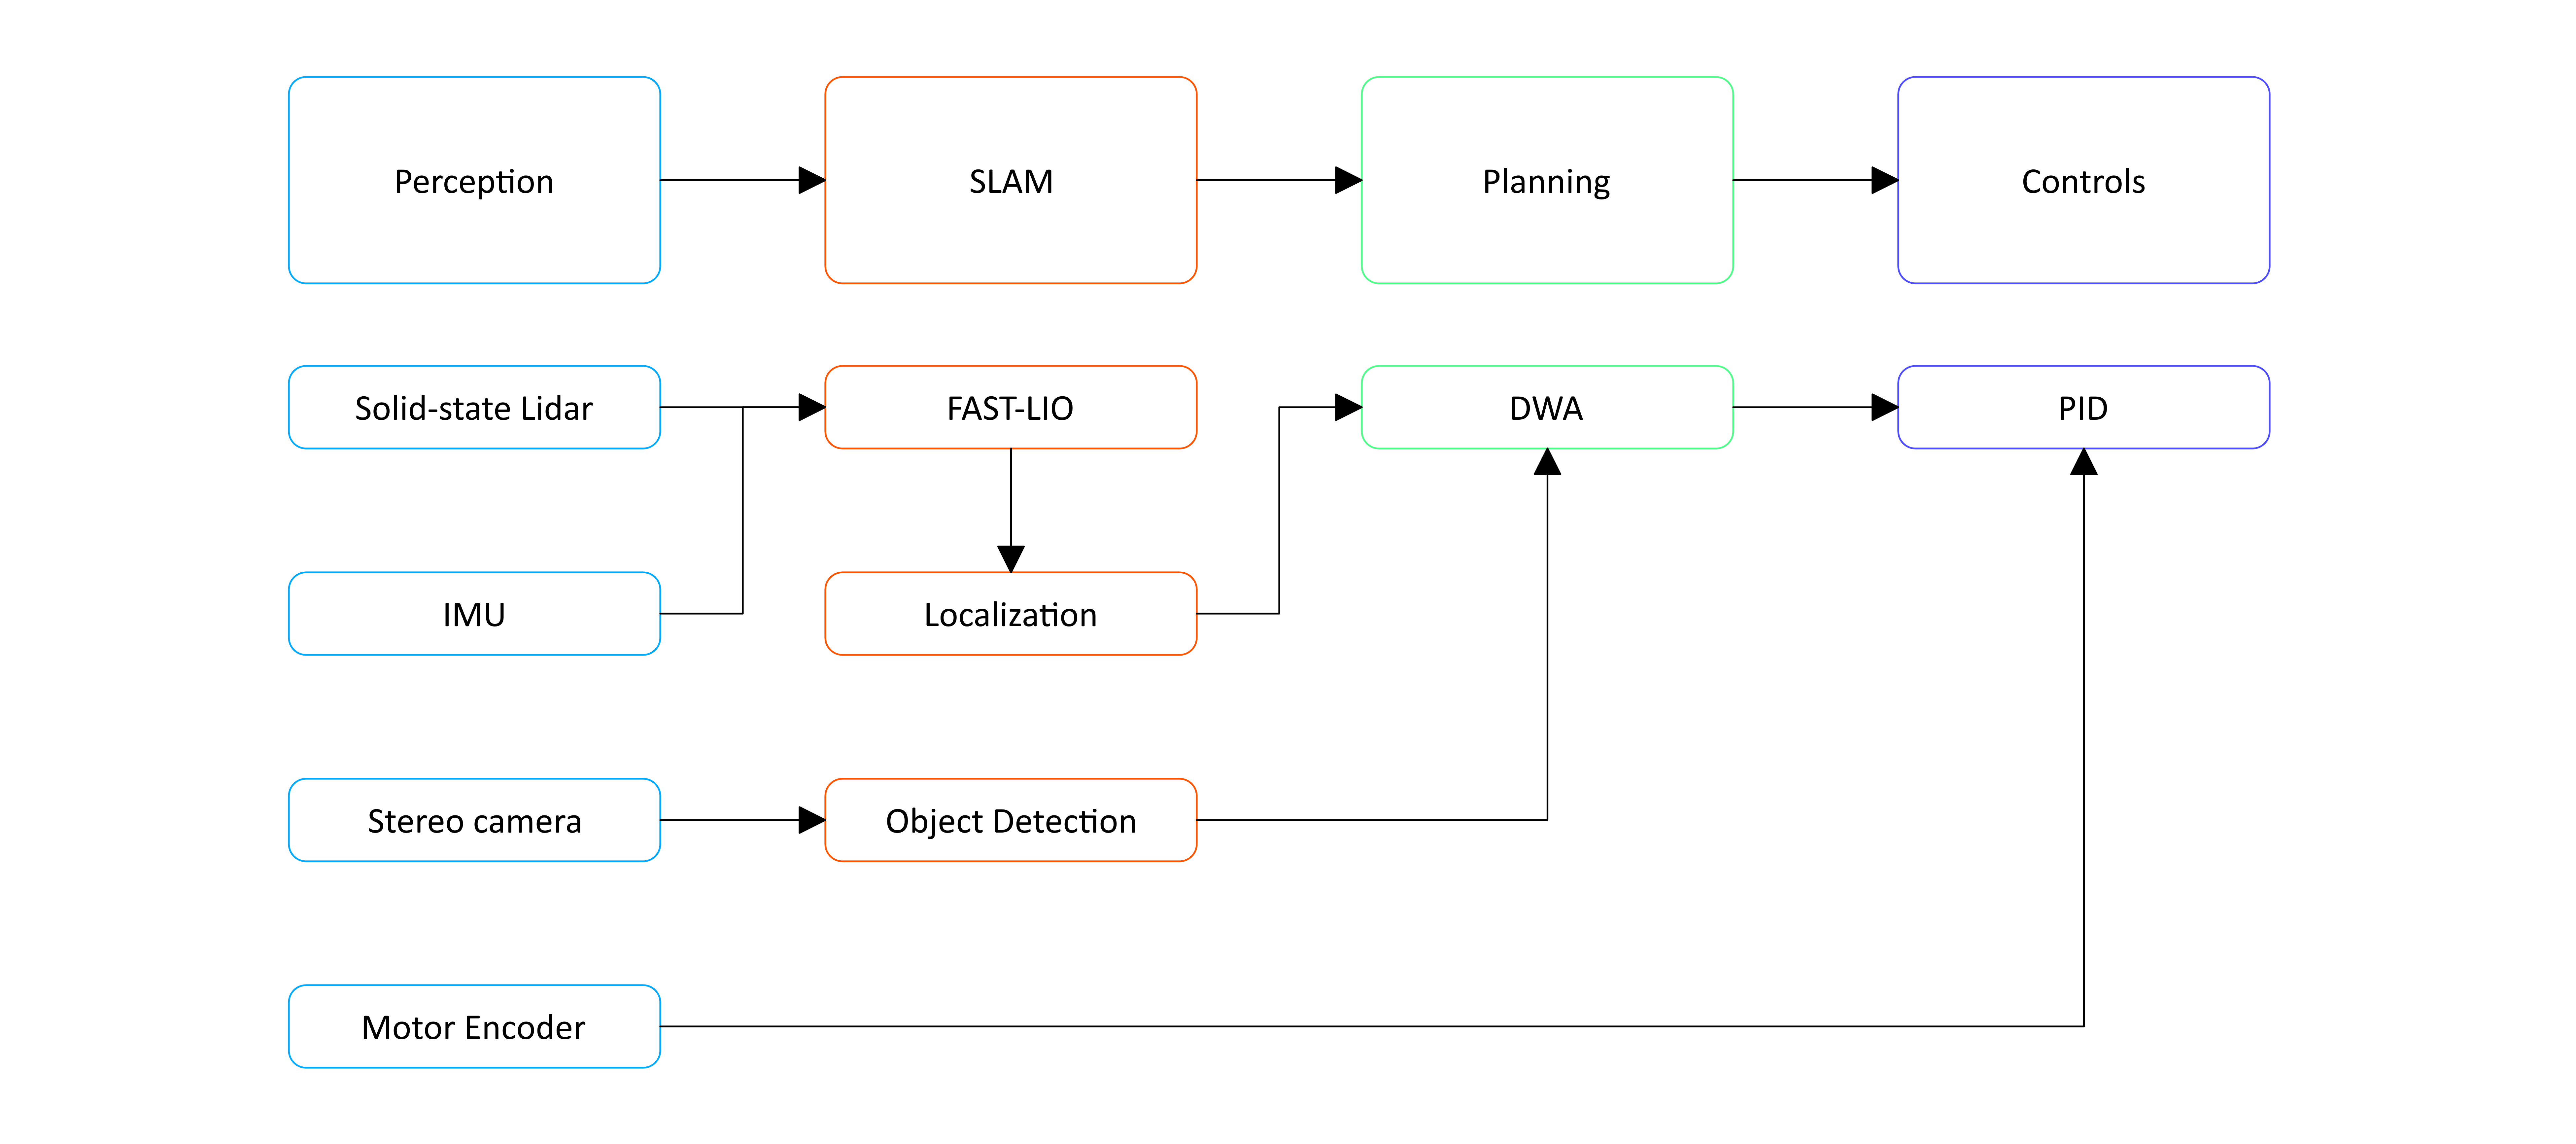
\includegraphics[width=0.9\textwidth]{flow_chart.png}
\caption{flow chart}
\end{figure*}
% \end{multicols}

%%%%%%%%%%%%% end figure %%%%%%%%%%%%%%%%%%%


%%%%%%%%%%%%%%%%%%%%%%%%%%%%%%%%%%%%%%%%%%%%%%%%%%%%%%%%%%%

%% Use title case for subsections and subsubsections (first letter of words capitalized)

\section{Results}

According to the experiment, the stereo camera’s object detection is relatively accurate even under indoor
envirnonment. The lidar’s point cloud is also shown to have a very good alignment with the depth map given by
the stereo camera.
%%%%%%%%%%%%%%%%%%%%%%%%%%%%%%%%%%%%%%%


%%%%% Acknowledgments %%%%%%%%%%%%%%%%%%%%%%%%%%%

\section*{Acknowledgments}
Place any acknowledgments here.


%%%  REFERENCES  %%%%%%%%%%%%%%%%%%%%%%%%%%%%%%%%
%%
%% Put your references into your .bib file in the usual way. Run latex once, bibtex once, then latex twice.
%% The asmeconf.bst style allows @inproceedings and @proceedings to include: 
%%		venue = {Location of Conference}, 
%%		eventdate = {Month, days},

\nocite{*}%% <=== Delete this line unless you want to typeset the entire contents of your .bib file!

\bibliographystyle{asmeconf}  %% .bst file following ASME conference format. Do not change.
\bibliography{asmeconf-sample}%% <=== change this to name of your bib file


%%%  APPENDICES  %%%%%%%%%%%%%%%%%%%%%%%%%%%%%%%%
\appendix

%% Note that appendices will be "numbered" A, B, C, ... etc. Use \section, not \section*
%% Equations will be numbered sequentially following those in the paper. Do not reset the equation counter.

%% Here we use the optional argument to control the pdf bookmark and prevent errors.
\newpage
\section[Camera Lidar Calibration]{Codes for Camera Lidar Calibration}\label{appendix:a}

\begin{minted}{python} 
import pyzed.sl as sl
import cv2
init_params = sl.InitParameters()
# runtime = sl.RuntimeParameters()
init_params.camera_resolution = sl.RESOLUTION.HD2K
# init_params.camera_fps = 30
zed = sl.Camera()
zed.open(init_params)
if not zed.is_opened():
  print("Opening ZED Camera...")
zed.grab(init_params)
image = sl.Mat()

zed.retrieve_image(image) # Retrieve the left image
cv2.imwrite("test.png", image.get_data())
\end{minted} 

%%%%%%%%%%%%%%%%%%%%%%%%%%%%%%%%%%%%%%%%%%%%%%%%%%%%%%%%%%%%%%%%%%%%%%%%%%%%%%%%%%%%%%%

\end{document}

